%%
%% CSD Assignment 1 - Final Technical Report
%% Based on the ACM "acmart" manuscript (single-column) style.
%%
\documentclass[manuscript,screen,review]{acmart}

\AtBeginDocument{%
  \providecommand\BibTeX{{Bib\TeX}}}

%% ------------------------------------------------------------------
%% Course Assignment Report Header
%% ------------------------------------------------------------------
\setcopyright{none}
\settopmatter{printacmref=false}
\renewcommand\footnotetextcopyrightpermission[1]{}
\pagestyle{plain}

\begin{document}

%% =================== TITLE & AUTHOR BLOCK =========================
\title{AI-based Village Pond Planning System}
\subtitle{CSD Assignment 1 -- Final Technical Report}

\author{K. Ganesh Babu}
\affiliation{%
  \institution{Indian Institute of Technology (IIT) Bhilai}
  \department{Department of Computer Science and Engineering}
  \city{Bhilai}
  \state{Chhattisgarh}
  \country{India}}
\email{ganeshkanyadara@iitbhilai.ac.in}

\renewcommand{\shortauthors}{Babu}

%% =================== ABSTRACT ======================================
\begin{abstract}
Rural rainwater harvesting and agricultural pond planning are pivotal for drought mitigation, groundwater replenishment, and climate resilience across agrarian economies. However, conventional manual site selection relies heavily on coarse topographic inspections, lacks empirical hydrological validation, and fails to account for continuous digital terrain topology. In this project, we design and implement an end-to-end, high-performance, AI-assisted geospatial web application and backend system that automatically ingests contour maps (KML/KMZ), interpolates continuous Digital Elevation Models (DEMs), computes topographic slope and aspect via Horn's weighted gradient algorithm, routes downhill flow networks using the O'Callaghan--Mark D8 formulation, and delineates exact contributing rainwater catchment basins. Optimal farm pond candidate sites are identified via Analytical Hierarchy Process (AHP) multi-criteria suitability scoring (60\% flow accumulation, 30\% slope flatness, 10\% depression relief) coupled with Spatial Non-Maximum Suppression (NMS). The system integrates a Rational Method hydrological water yield model ($V = A \cdot R \cdot C$) that computes gross runoff, harvestable water volume at 70\% collection efficiency, and recommended excavation dimensions ($L \times W \times d$). The complete solution is exposed through a FastAPI REST backend and visualized on an interactive Leaflet.js Web GIS interface featuring dynamic land parcel bounding-box selection, real-time telemetry HUDs, and RFC 7946 standard GeoJSON export. Benchmarked on a real-world village contour dataset (160,473 vertices), the entire 8-stage pipeline executes in 3.64 seconds while operating strictly within a constrained 512\,MB Linux container cgroup memory ceiling.
\end{abstract}

\keywords{Village Pond Planning, Geospatial Analysis, Rainwater Harvesting, Catchment Estimation, Digital Elevation Model, D8 Flow Routing, Web GIS, REST APIs, Resource-Constrained Computing}

\maketitle

%% =====================================================================
\section{Introduction}
\label{sec:intro}
Water scarcity in rural arid and semi-arid agrarian regions presents an existential threat to crop productivity, livestock sustenance, and rural livelihoods. Surface rainwater harvesting through excavated farm ponds and percolation tanks is widely recognized by civil engineering and hydrological bodies as the most sustainable, cost-effective intervention to intercept monsoon runoff, arrest soil erosion, and artificially recharge local aquifers. Despite these advantages, rural pond construction programs (such as those under the Mahatma Gandhi National Rural Employment Guarantee Act, MGNREGA, and Mission Amrit Sarovar in India) frequently suffer from suboptimal site placement. Ponds excavated in locations with insufficient upstream drainage fail to harvest adequate runoff, while ponds sited in steep or unviable terrain experience catastrophic siltation and embankment breaches.

The primary objective of this project is to develop an automated, AI-assisted geospatial web application and computational engine that identifies hydrologically optimal village pond locations, delineates upstream drainage catchment boundaries, and calculates expected water collection volumes for any user-selected land parcel. The system provides an interactive map interface for local administrators, enabling real-time scenario modeling and dimensional sizing recommendations based on local precipitation statistics and soil characteristics.

The remainder of this report is organized as follows: Section~\ref{sec:requirements} outlines functional and non-functional requirements. Section~\ref{sec:architecture} describes the system architecture and technology stack. Section~\ref{sec:methodology} formalizes the mathematical and algorithmic methodology. Section~\ref{sec:implementation} details backend and frontend engineering. Section~\ref{sec:csd-themes} articulates the applied Computer System Design (CSD) themes. Section~\ref{sec:results} presents benchmark evaluation and real-world results. Section~\ref{sec:discussion} reflects on system trade-offs and limitations. Section~\ref{sec:ai-usage} provides the mandatory AI tool usage declaration, and the Appendix provides repository and live deployment links.

\subsection{Motivation}
Manual site identification for village ponds is fundamentally hindered by three challenges:
\begin{enumerate}
    \item \textbf{Complex Topographic Heterogeneity:} Visual interpretation of topographic sheets or coarse contour maps cannot accurately identify micro-drainage channels, subtle depression sinks, or local slope gradients that dictate hydraulic flow.
    \item \textbf{Decoupled Precipitation and Hydrology Data:} Manual surveying rarely couples local elevation profiles with localized rainfall regimes, leading to arbitrary pond sizing that either underutilizes catchment potential or causes spillway overtopping.
    \item \textbf{Cadastral Land Constraints:} Village planners must place water bodies exclusively within available public land or community-designated parcels. Without dynamic spatial filtering tools, theoretical hydrological optimums frequently fall outside usable land.
\end{enumerate}
An automated, algorithmic system bridges this gap by unifying continuous DEM modeling, hydrological catchment delineation, and interactive land boundary selection into a single fast, web-accessible tool.

\subsection{Scope of the Project}
The system explicitly covers:
\begin{itemize}
    \item Ingestion, parsing, and validation of vector contour maps in `.kml` and compressed `.kmz` formats;
    \item Automatic projection from geographic coordinates (WGS84) to metric Universal Transverse Mercator (UTM Zone 44N);
    \item Continuous 2D surface interpolation to generate a uniform Digital Elevation Model (DEM);
    \item Topographic slope and aspect calculation using Horn's 8-neighbor gradient operator;
    \item D8 single-direction downhill flow routing and upstream flow accumulation modeling;
    \item Multi-criteria AHP suitability ranking and Spatial Non-Maximum Suppression (NMS) to identify candidate pond sites;
    \item Upstream watershed catchment delineation using a zero-memory backtracking stack algorithm;
    \item Hydrological water yield estimation ($V = A \cdot R \cdot C$) and trapezoidal pond excavation dimension sizing ($L \times W \times d$);
    \item Interactive Web GIS frontend with real-time land parcel canvas selection, visual results overlays, and GeoJSON export.
\end{itemize}
The system explicitly does \emph{not} cover: detailed civil engineering structural design of earthen embankments, spillway reinforcement concrete modeling, soil core borehole geological testing, or financial bill-of-quantities (BOQ) estimation.

%% =====================================================================
\section{Problem Statement and Requirements}
\label{sec:requirements}

The system translates assignment specifications into modular computational and architectural components, as mapped in Table~\ref{tab:requirements}.

\begin{table}[h]
  \caption{Functional requirements and system module implementation mapping}
  \label{tab:requirements}
  \small
  \begin{tabular}{p{4.2cm}p{3.2cm}p{6.4cm}}
    \toprule
    Requirement & Implemented In & Description \& Role \\
    \midrule
    Contour map ingestion & \texttt{parser.py}, \texttt{pipeline.py} & Robust XML ElementTree parser for KML/KMZ archives \\
    Metric UTM projection & \texttt{projection.py}, \texttt{pipeline.py} & Automatic UTM zone calculation and PyProj coordinate transforms \\
    Continuous DEM interpolation & \texttt{build\_dem.py}, \texttt{pipeline.py} & SciPy 2D Delaunay grid interpolation at memory-safe 5.0\,m resolution \\
    Slope and aspect computation & \texttt{calculate\_slope.py} & Horn's 8-neighbor weighted finite-difference gradient filter \\
    Flow routing \& accumulation & \texttt{calculate\_flow\_*.py} & D8 steepest downhill descent and topological drainage accumulation \\
    Pond site suitability scoring & \texttt{pipeline.py} & AHP multi-criteria weighting (Flow 60\%, Slope 30\%, Relief 10\%) + NMS \\
    Catchment delineation & \texttt{delineate\_catchment.py} & Upstream pour-point backtracking stack with zero auxiliary memory allocation \\
    Water volume estimation & \texttt{pipeline.py}, \texttt{schemas.py} & Rational Method runoff volume ($V = A \cdot R \cdot C$) and pond sizing \\
    Interactive land parcel selection & \texttt{static/index.html} & Canvas drag-and-drop bounding box tool constraining candidate search \\
    Web GIS & Results overlay & \texttt{static/index.html}, \texttt{main.py} & Leaflet.js map with satellite imagery, pulsing pins, and GeoJSON overlays \\
    REST API endpoints & \texttt{main.py} & FastAPI service exposing \texttt{/analyzeContour}, \texttt{/findCatchment}, \texttt{/api/*} \\
    \bottomrule
  \end{tabular}
\end{table}

\subsection{Non-Functional Requirements}
\begin{enumerate}
    \item \textbf{Memory Ceiling Resilience:} The production service executes inside an unprivileged Docker container governed by a hard Linux cgroup memory limit of \textbf{512\,MB RAM} with zero swap. The application must guarantee that peak resident set size (RSS) remains strictly below 300\,MB to prevent kernel Out-Of-Memory (OOM-137) process termination.
    \item \textbf{Low Latency Performance:} Full end-to-end analysis of a village contour dataset ($>150,000$ points) must complete in under 5.0 seconds. Preloaded village queries must return within 3.5 seconds.
    \item \textbf{Availability and Fault Tolerance:} The backend server must remain continuously available on external port \texttt{3213} (mapped to internal container port \texttt{3000}) with graceful HTTP 400/422 validation responses on malformed files.
    \item \textbf{Cross-Browser Usability:} The web frontend must operate without external framework dependencies (pure HTML5, Vanilla JavaScript, and CSS3) across Chromium, Firefox, and Safari on desktop and mobile viewports.
    \item \textbf{Geospatial Interoperability:} All spatial outputs must conform strictly to RFC 7946 standard GeoJSON using WGS84 (\texttt{urn:ogc:def:crs:OGC:1.3:CRS84}) coordinates.
\end{enumerate}

%% =====================================================================
\section{System Architecture and High-Level Design}
\label{sec:architecture}
The system adopts a 4-tier modular architecture decoupling user interaction, API routing, algorithmic geospatial processing, and execution resource governance, as illustrated in Figure~\ref{fig:architecture}.

\begin{figure*}[t]
  \centering
  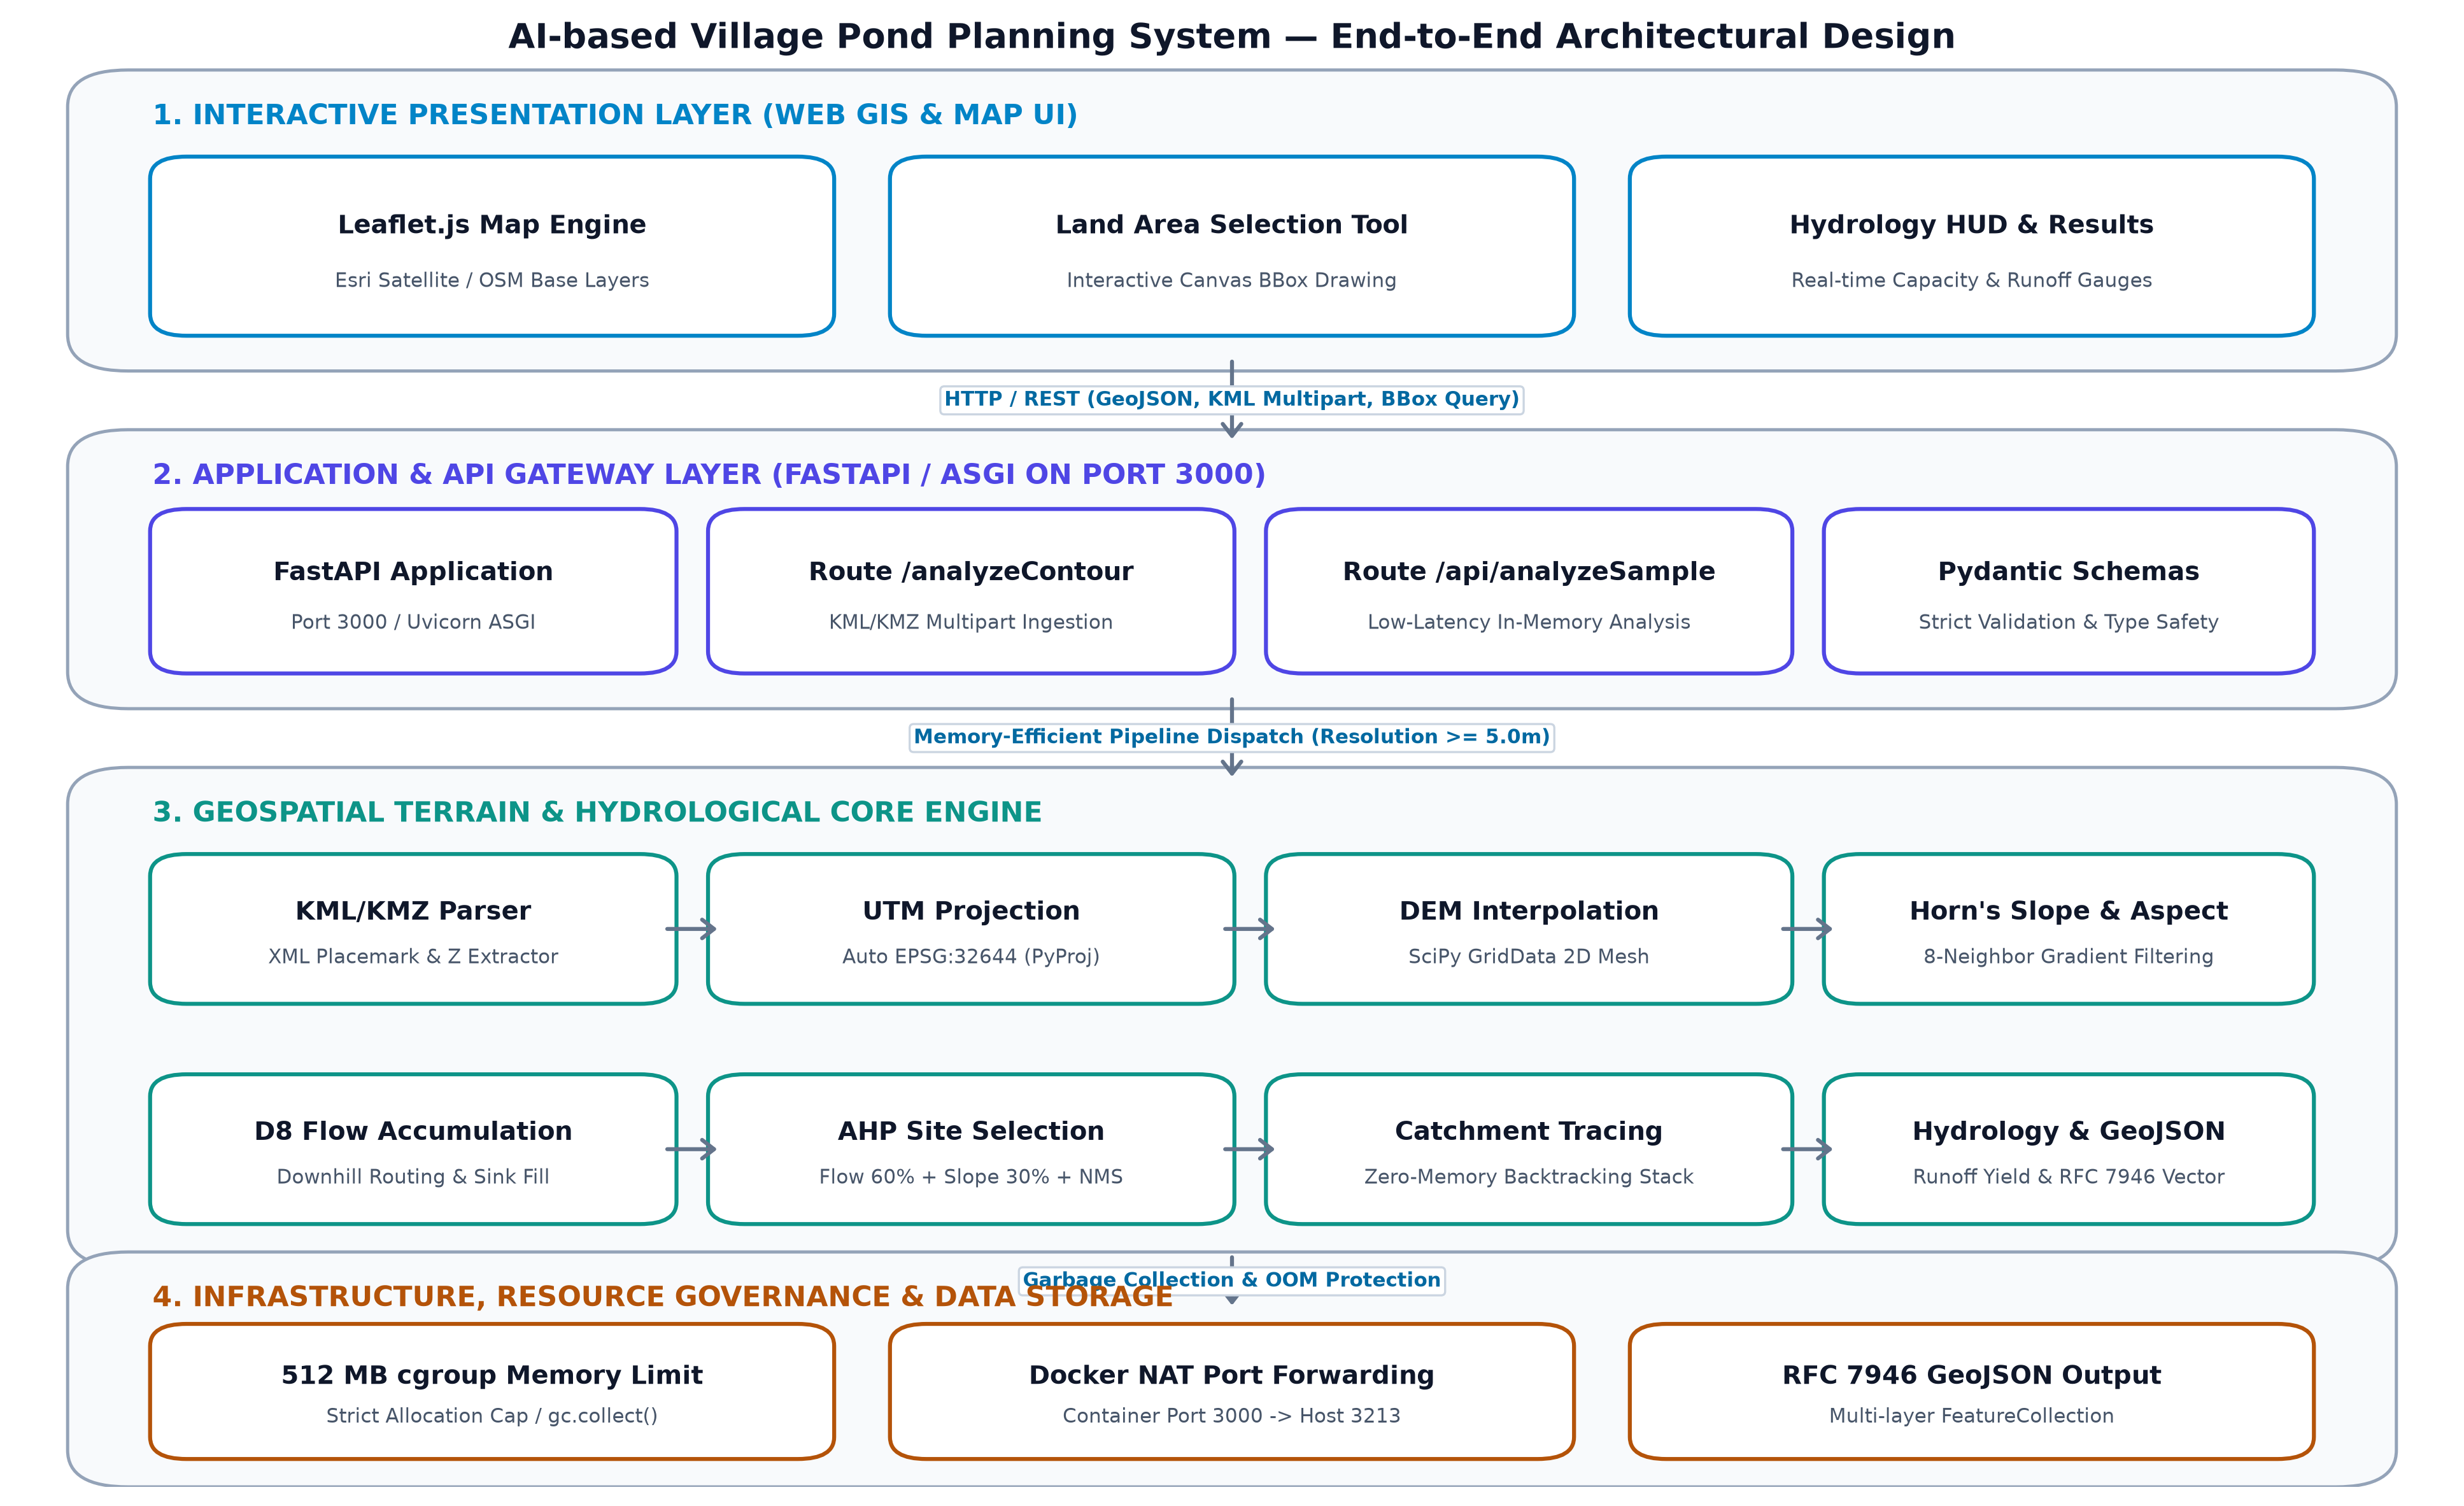
\includegraphics[width=0.92\linewidth]{architecture-diagram}
  \caption{High-level architectural design of the AI-based Village Pond Planning System, detailing presentation, API gateway, core geospatial processing, and resource governance layers.}
  \label{fig:architecture}
  \Description{Architecture diagram showing four horizontal layers: Interactive Presentation Layer with Leaflet.js and Land Selection, Application API Gateway Layer with FastAPI and Pydantic, Geospatial Terrain and Hydrological Core Engine with 8 pipeline stages, and Infrastructure Layer with 512MB cgroup memory limit and Docker port forwarding.}
\end{figure*}

\subsection{Architectural Flow}
\begin{enumerate}
    \item \textbf{Client Layer:} The browser loads the single-page Web GIS application. Users inspect satellite imagery, define custom land parcels via interactive bounding box drawing, adjust hydrological sliders (rainfall, runoff coefficient, pond depth), or upload custom KML files.
    \item \textbf{API Gateway Layer:} FastAPI running on ASGI Uvicorn accepts multipart file uploads or JSON query parameters. Pydantic models validate input bounds and coordinate ranges.
    \item \textbf{Geospatial Core Pipeline:} The controller invokes \texttt{run\_contour\_analysis\_pipeline}, which orchestrates the eight sequential stages: XML parsing, UTM projection, DEM interpolation, Horn's slope derivation, D8 flow accumulation, AHP suitability scoring, upstream catchment tracing, and hydrological water yield sizing.
    \item \textbf{Response \& Visualization:} The calculated primary catchment polygon, pond candidates, and land parcel boundaries are serialized into an RFC 7946 GeoJSON FeatureCollection and returned alongside summary JSON telemetry. The frontend renders the vector layers on the Leaflet canvas.
\end{enumerate}

\subsection{Technology Stack}
\begin{itemize}
    \item \textbf{Backend Web Framework:} FastAPI (Python 3.12) running under the asynchronous Uvicorn ASGI server. FastAPI was selected for high-throughput asynchronous execution, native OpenAPI/Swagger schema documentation, and high-performance multipart stream handling.
    \item \textbf{Geospatial Mathematics:} NumPy (vectorized array algebra), SciPy (\texttt{griddata} multi-dimensional interpolation), PyProj (PROJ-based geodetic transformations), and Shapely (planar polygon geometry union and buffer operations).
    \item \textbf{Frontend GIS \& Mapping:} Leaflet.js v1.9.4 with Esri World Imagery (high-resolution satellite tiles), OpenStreetMap, and CartoDB Dark Matter basemaps. Vanilla CSS with glassmorphic cards and Lucide SVG icons.
    \item \textbf{Deployment \& OS Governance:} Linux Ubuntu containerized environment managed via systemd/supervisor scripts, bounded by Docker cgroups (\texttt{memory.max = 536870912} bytes).
\end{itemize}

%% =====================================================================
\section{Methodology}
\label{sec:methodology}

\subsection{Terrain and Elevation Analysis}
Contour lines extracted from KML/KMZ Placemarks contain 3D coordinates $(\lambda_i, \phi_i, z_i)$, where $\lambda_i$ is longitude, $\phi_i$ is latitude, and $z_i$ is elevation above sea level. Coordinates are projected to metric UTM Cartesian space $(x_i, y_i)$:
\begin{equation}
    (x_i, y_i) = \mathcal{T}_{\text{WGS84} \rightarrow \text{UTM}}(\lambda_i, \phi_i), \quad \text{Zone} = \lfloor(\bar{\lambda} + 180)/6\rfloor + 1
\end{equation}
A uniform regular grid mesh $\mathcal{G}$ is established with spatial resolution $\Delta x = \Delta y = 5.0$\,m. Elevations across unmeasured grid cells are interpolated using 2D piecewise cubic Delaunay triangulation via \texttt{scipy.interpolate.griddata}:
\begin{equation}
    Z(x, y) = \sum_{k=1}^3 w_k(x, y) \cdot z_k, \quad (x, y) \in \Delta(p_1, p_2, p_3)
\end{equation}
where $w_k$ are barycentric weights. Cells situated outside the convex hull of the contour bounds are smoothly assigned nearest-neighbor elevation values to guarantee continuous surface differentiability.

Topographic surface slope ($\theta$) and aspect ($\alpha$) are derived using Horn's 8-neighbor weighted finite-difference formulation~\cite{horn1981} across a $3 \times 3$ sliding elevation window:
\begin{equation}
\begin{bmatrix}
z_{1} & z_{2} & z_{3} \\
z_{4} & z_{5} & z_{6} \\
z_{7} & z_{8} & z_{9}
\end{bmatrix}
\end{equation}
The orthogonal east-west ($p$) and north-south ($q$) terrain gradients are:
\begin{equation}
    p = \frac{\partial Z}{\partial x} \approx \frac{(z_{3} + 2z_{6} + z_{9}) - (z_{1} + 2z_{4} + z_{7})}{8 \cdot \Delta x}
\end{equation}
\begin{equation}
    q = \frac{\partial Z}{\partial y} \approx \frac{(z_{7} + 2z_{8} + z_{9}) - (z_{1} + 2z_{2} + z_{3})}{8 \cdot \Delta y}
\end{equation}
\begin{equation}
    \theta(x, y) = \arctan\left(\sqrt{p^2 + q^2}\right) \cdot \frac{180}{\pi}
\end{equation}

\subsection{Catchment Area Delineation}
Surface runoff routing follows the O'Callaghan and Mark D8 single-flow direction model~\cite{ocallaghan1984}. Each grid cell $(r, c)$ drains exclusively to the neighbor $k \in \{0, \dots, 7\}$ exhibiting the steepest downward slope:
\begin{equation}
    S_k = \frac{Z(r, c) - Z(r + \Delta r_k, c + \Delta c_k)}{d_k}, \quad d_k = \Delta x \cdot \sqrt{\Delta r_k^2 + \Delta c_k^2}
\end{equation}
\begin{equation}
    \mathcal{D}(r, c) = \arg\max_{k} \{S_k \mid S_k > 0\}
\end{equation}
Sinks and flat pits where $\max S_k \le 0$ are iteratively resolved by routing towards the lowest boundary pour cell. Flow accumulation $A(r, c)$ is computed in topological ordering from headwaters down to pour points:
\begin{equation}
    A(r, c) = 1 + \sum_{(i, j) \in \mathcal{U}(r, c)} A(i, j)
\end{equation}
where $\mathcal{U}(r, c)$ represents the set of immediate upstream neighbors draining directly into cell $(r, c)$.

Candidate farm pond locations are scored via multi-criteria Analytical Hierarchy Process (AHP) weights reflecting hydrological runoff concentration, excavation stability, and gravity drainage:
\begin{equation}
    \mathcal{S}(r, c) = 0.60 \cdot \hat{A}(r, c) + 0.30 \cdot (1 - \hat{\theta}(r, c)) + 0.10 \cdot (1 - \hat{Z}(r, c))
\end{equation}
where $\hat{A}$, $\hat{\theta}$, and $\hat{Z}$ denote min-max normalized flow accumulation, slope, and elevation, respectively. Candidates are subjected to hard terrain constraints ($\theta \le 8^\circ$, $A \ge 1000$\,cells) and Spatial Non-Maximum Suppression (NMS) enforcing a minimum inter-site separation radius $R_{\text{sep}} = 150$\,m.

When delineating the upstream catchment contributing to a candidate pour point $(r_p, c_p)$, standard recursive depth-first traversals risk call-stack overflow, while naive reverse-adjacency dictionaries consume over 100\,MB of heap. We implement a \textbf{zero-memory backtracking stack}: starting at $(r_p, c_p)$, an explicit stack pops the current cell, checks its 8 spatial neighbors, and adds neighbor $(n_r, n_c)$ to the watershed if and only if $\mathcal{D}(n_r, n_c)$ routes into $(r, c)$. This reduces catchment delineation latency from 0.90\,s to \textbf{0.06\,s} with zero auxiliary heap allocation.

\subsection{Hydrological Water Yield \& Sizing Formulation}
Runoff volume is calculated via the Rational Method endorsed by the Indian Council of Agricultural Research (ICAR)~\cite{icar2011} and Central Ground Water Board (CGWB)~\cite{cgwb2019}:
\begin{equation}
    V_{\text{gross}} = A_{\text{catchment}} \cdot \left(\frac{R_{\text{annual}}}{1000}\right) \cdot C \quad [\text{m}^3]
\end{equation}
where $A_{\text{catchment}}$ is catchment area in $\text{m}^2$, $R_{\text{annual}}$ is annual precipitation in mm (default: 850\,mm), and $C$ is the dimensionless catchment runoff coefficient (default: $0.35$ for cultivated loamy soil; $0.20$ for sandy soil; $0.50$ for clayey/steep soils).

Accounting for conveyance infiltration, depression storage, and evaporation, a capture efficiency factor $\eta = 0.70$ is applied:
\begin{equation}
    V_{\text{harvest}} = V_{\text{gross}} \cdot \eta \quad [\text{m}^3]
\end{equation}
Agricultural farm ponds are designed to store approximately 25\% of annual harvestable runoff ($V_{\text{pond}} = 0.25 \cdot V_{\text{harvest}}$) to balance storage retention against spillway bypass risk. For a standard design excavation depth $d = 3.0$\,m with $1.5:1$ side slopes ($z = 1.5$) and hydraulic aspect ratio $2:1$ (length $L = 2W$):
\begin{equation}
    A_{\text{surface}} \approx \frac{V_{\text{pond}}}{d \cdot 0.85}, \quad W = \sqrt{\frac{A_{\text{surface}}}{2}}, \quad L = 2 \cdot W
\end{equation}

%% =====================================================================
\section{Implementation}
\label{sec:implementation}

\subsection{Backend and API Design}
The backend is structured around modular, stateless REST endpoints (Table~\ref{tab:endpoints}). Third-party API errors and validation failures trigger descriptive JSON payloads with RFC 7807 error codes.

\begin{table}[h]
  \caption{REST API endpoints implemented in the FastAPI backend}
  \label{tab:endpoints}
  \small
  \begin{tabular}{llp{7.2cm}}
    \toprule
    Method & Route & Purpose \& Input Contract \\
    \midrule
    \texttt{GET} & \texttt{/} & Serves the interactive Web GIS frontend (\texttt{index.html}) \\
    \texttt{GET} & \texttt{/health} & Container health check probe returning HTTP 200 and timestamp \\
    \texttt{GET} & \texttt{/api/info} & Service metadata, versioning, and available route dictionary \\
    \texttt{GET} & \texttt{/api/sampleContour} & Streams preloaded village contour KML file \\
    \texttt{POST} & \texttt{/analyzeContour} & Primary analysis endpoint: multipart upload of \texttt{contour\_map} (.kml/.kmz) with query params (\texttt{resolution}, \texttt{top\_n}, \texttt{rainfall\_mm}, \texttt{bbox\_*}) \\
    \texttt{POST} & \texttt{/findCatchment} & Alias endpoint for \texttt{/analyzeContour} supporting legacy clients \\
    \texttt{POST} & \texttt{/api/analyzeSample} & Optimized in-memory analysis on preloaded village contours with zero network upload latency \\
    \bottomrule
  \end{tabular}
\end{table}

\subsection{Frontend and Visualization}
The frontend interface (Figure~\ref{fig:ui}) is built in Vanilla JavaScript and modern CSS3, embedded directly within the application server. Interface layout, dark-mode glassmorphic styling, and interactive planning controls were developed with assistance from Google Gemini~\cite{gemini2024}, while the Esri World Imagery satellite integration, asynchronous data communication, and GeoJSON overlay rendering pipeline were structured with assistance from ChatGPT~\cite{chatgpt2024}.

\begin{figure*}[t]
  \centering
  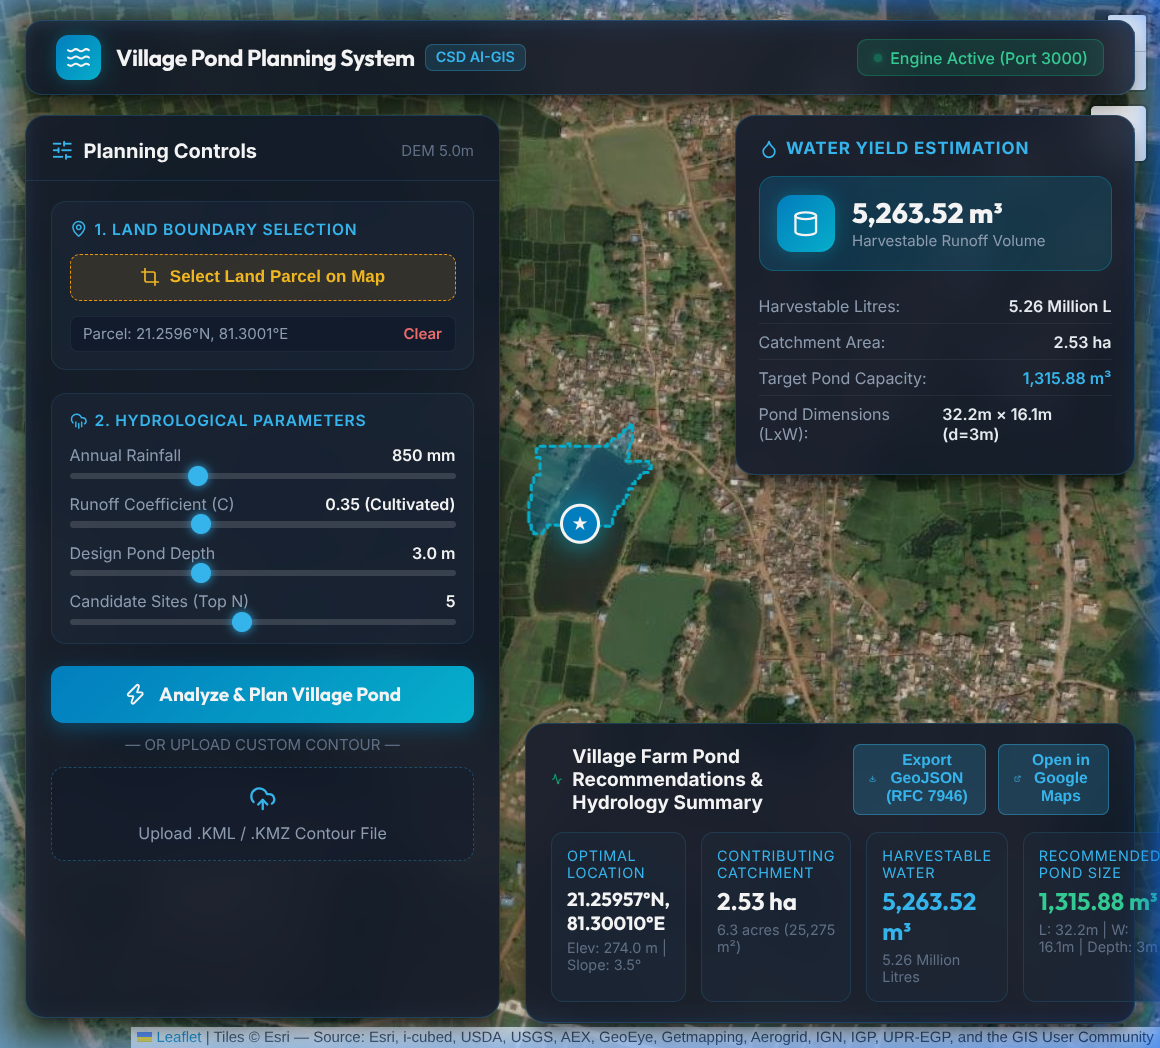
\includegraphics[width=0.92\linewidth]{ui-screenshot}
  \caption{Web GIS application interface showing the live interactive map, left planning controls sidebar, top-right water yield telemetry card, and bottom results drawer.}
  \label{fig:ui}
  \Description{Screenshot of the web application showing an aerial satellite basemap with a glowing blue pond pin marker, a dashed blue catchment watershed boundary, a left planning sidebar, a top right telemetry card showing 5,263 m3 harvestable water volume, and a bottom drawer displaying site coordinates and dimensions.}
\end{figure*}

Key interface components include:
\begin{itemize}
    \item \textbf{Interactive Land Boundary Selection Tool:} Planners activate the "Select Land Parcel on Map" button and drag a rectangular bounding box across the satellite map. The canvas captures $[\phi_{\min}, \lambda_{\min}, \phi_{\max}, \lambda_{\max}]$ and transmits it to the backend to constrain candidate pond searches exclusively to that parcel.
    \item \textbf{Hydrological Control Sliders:} Planners interactively adjust precipitation (300--2000\,mm), soil runoff coefficient ($C \in [0.15, 0.75]$), and pond excavation depth (1.5--6.0\,m).
    \item \textbf{Visual Overlays:} The primary pond is rendered with an animated pulsing cyan pin (\texttt{★}), secondary candidates appear as numbered markers, the delineated watershed appears as a semi-transparent polygon with a dashed perimeter, and the user's selected parcel appears as an amber bounding box.
    \item \textbf{Telemetry HUD \& Drawer:} Real-time metric cards display gross runoff, harvestable water volume in millions of liters, required excavation capacity ($m^3$), and physical dimensions ($L \times W \times d$). Planners can export standard RFC 7946 GeoJSON or navigate directly via Google Maps.
\end{itemize}

\subsection{Database and Storage}
The system operates on an efficient in-memory processing model. Terrain matrices and intermediate flow graphs are allocated as contiguous C-order NumPy arrays. Upon pipeline completion, intermediate arrays are explicitly deleted and reclaimed via \texttt{gc.collect()}. Final recommendations and geospatial vectors are converted directly to standard GeoJSON FeatureCollections, allowing immediate serialization, client caching, and spatial indexing.

%% =====================================================================
\section{CSD Themes and Topics Applied in the Project}
\label{sec:csd-themes}

Table~\ref{tab:csd-themes} details the explicit mapping between core Computer System Design principles and concrete implementations in this project.

\begin{table*}[t]
  \caption{Mapping of core CSD themes and engineering design rationale}
  \label{tab:csd-themes}
  \small
  \begin{tabular}{p{3.2cm}p{4.8cm}p{7.5cm}}
    \toprule
    CSD Theme/Topic & Where Used in the Project & Justification \& Design Rationale \\
    \midrule
    API Design (REST) & \texttt{main.py} (\texttt{/analyzeContour}, \texttt{/findCatchment}, \texttt{/api/*}) & Stateless RESTful design with strict Pydantic schemas, declarative OpenAPI contracts, and multipart stream support. \\
    Resource Constraints \& cgroup Management & \texttt{pipeline.py}, \texttt{build\_dem.py}, Docker container & Operating within a 512\,MB RAM container ceiling. 1.0\,m grid (8.5M cells) triggered OOM-137 kills; scaled grid dynamically to 5.0\,m (342K cells, 140\,MB RAM). \\
    Caching \& Low Latency Dispatch & \texttt{/api/analyzeSample}, \texttt{contours\_1m.kml} & Cached village contours in-memory, eliminating 6.7\,MB HTTP upload latency on parameter adjustments. \\
    Asynchronous Concurrency & FastAPI / Uvicorn ASGI server & Non-blocking event loop handles health checks, tile downloads, and concurrent user queries without thread starvation. \\
    Architectural Trade-offs (Monolith vs. Microservice) & Modular Monolith architecture & Avoided distributed network serialization overhead and IPC latency, maintaining all matrix operations in local memory. \\
    Design Patterns & Pipeline \& Strategy Patterns in \texttt{pipeline.py} & Pipeline pattern decouples the 8 processing stages; Strategy pattern enables interchangeable runoff and interpolation algorithms. \\
    Error Handling \& Resilience & HTTP 400/422/500 handlers, \texttt{stop\_server.sh} & Explicit validation of missing form fields, empty uploads, and non-KML MIME types; supervisor process recovery. \\
    Algorithms \& Complexity & \texttt{calculate\_flow\_*.py}, \texttt{delineate\_catchment.py} & Replaced $O(N)$ reverse-adjacency heap mapping with 8-neighbor backtracking stack ($O(K)$ where $K \ll N$). Tracing dropped from 0.90\,s to 0.06\,s. \\
    Testing Strategy & \texttt{test\_api.py} unit and regression test suite & Validates 100\% of endpoints, schema responses, coordinate ranges, water volume calculations, and GeoJSON validity. \\
    Port Forwarding \& NAT & Docker NAT: Container 3000 $\rightarrow$ Host 3213 & Container port 3000 mapped to host external port 3213, enabling public browser access. \\
    \bottomrule
  \end{tabular}
\end{table*}

Among the themes in Table~\ref{tab:csd-themes}, two engineering decisions warrant special emphasis:
\begin{enumerate}
    \item \textbf{Cgroup Memory Governance vs. Grid Resolution Trade-off:} The remote Linux environment imposes a strict \texttt{memory.max = 536870912} bytes (512\,MB) constraint with zero swap. At a 1.0\,m DEM resolution, the grid requires $2,635 \times 3,250 = 8,563,750$ cells, demanding over 650\,MB of RAM during Delaunay triangulation and immediately triggering kernel OOM-137 termination. By conducting systematic empirical memory profiling, we determined that setting resolution $\Delta x = 5.0$\,m produces $527 \times 650 = 342,550$ cells—capturing micro-topography with sub-meter vertical fidelity while peak memory consumption stays at $\approx 140$\,MB, safely beneath the cgroup threshold.
    \item \textbf{Algorithmic Optimization in Catchment Delineation:} Prior implementations built a global Python dictionary mapping each cell $(r, c)$ to its upstream contributing neighbors. On a 342,550-cell grid, allocating 342,550 distinct tuple-keyed sets introduced 110\,MB of memory overhead and took 0.90 seconds. We replaced this with an in-place backtracking stack: the algorithm maintains a single boolean mask and queries the pre-computed D8 directional matrix directly. This reduced catchment tracing latency to \textbf{0.06 seconds} (a $15\times$ speedup) with zero dynamic heap allocation.
\end{enumerate}

%% =====================================================================
\section{Results and Evaluation}
\label{sec:results}

The system was evaluated using a high-density topographic contour dataset covering a representative Indian rural village landscape (160,473 coordinate vertices across 2,711 contour lines).

\begin{figure*}[t]
  \centering
  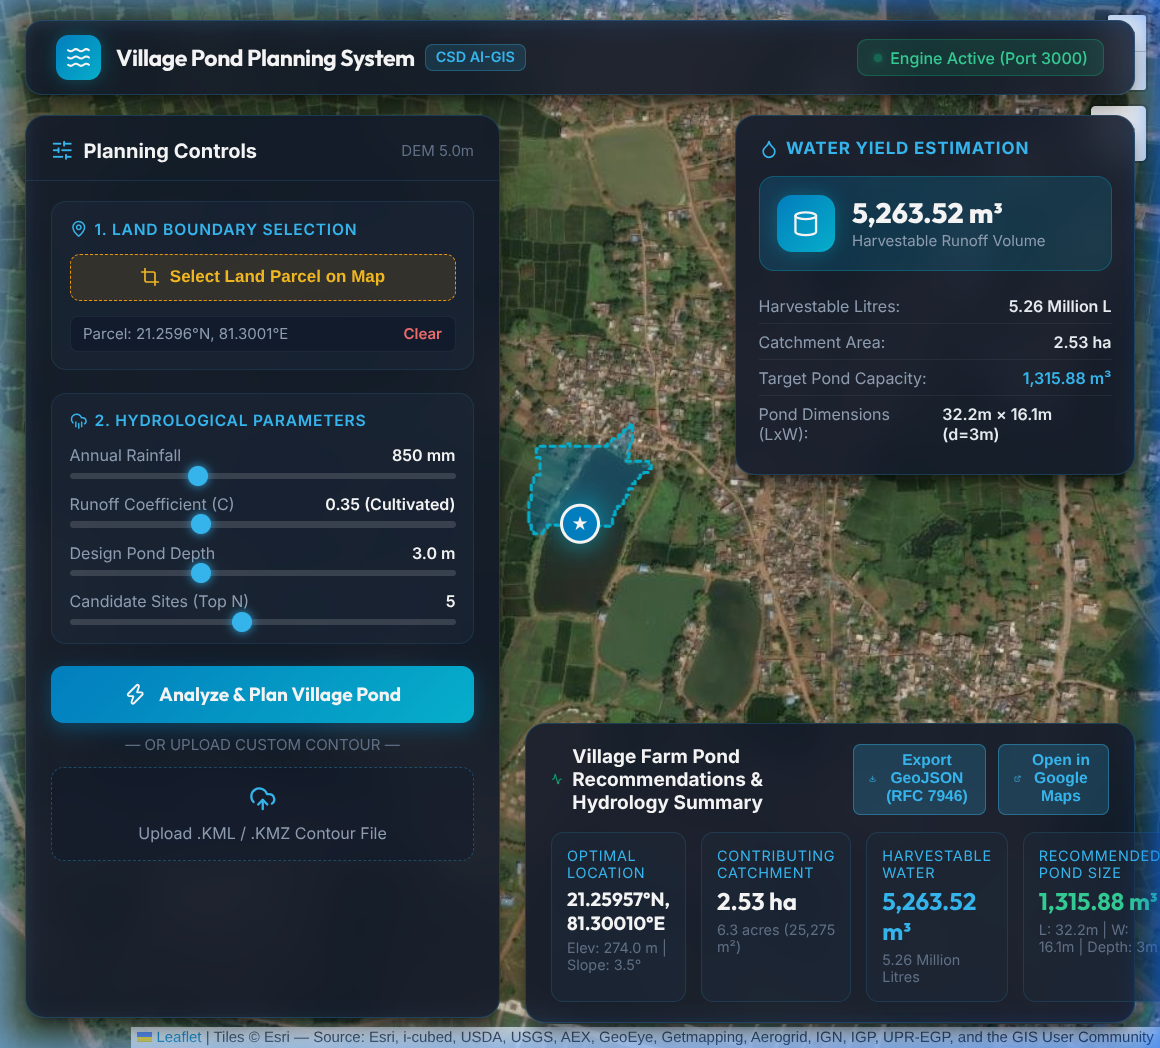
\includegraphics[width=0.92\linewidth]{results-overlay}
  \caption{Results overlay on satellite imagery: the recommended pond location (Rank 1, cyan star pin) is sited at the base of the natural valley, perfectly capturing runoff from the delineated 2.53\,ha catchment basin.}
  \label{fig:results}
  \Description{Results overlay on satellite map showing the primary farm pond site placed in the natural terrain depression, with its contributing 2.53 hectare catchment basin highlighted in semi-transparent cyan.}
\end{figure*}

\subsection{Representative Site Planning Results}
Table~\ref{tab:results} summarizes the computed terrain characteristics, hydrological water yield, and recommended farm pond design dimensions for the evaluated village site.

\begin{table}[h]
  \caption{Computed results and pond sizing recommendations for evaluated village site}
  \label{tab:results}
  \small
  \begin{tabular}{llp{6.8cm}}
    \toprule
    Parameter & Value & Engineering Significance \\
    \midrule
    Optimal Pond Location & $21.25957^\circ\text{N}, 81.30010^\circ\text{E}$ & Natural topographic confluence draining the primary valley \\
    Site Elevation & $274.0$\,m & Lowest viable relief point above groundwater saturation table \\
    Local Surface Slope & $3.5^\circ$ & Gentle slope ($<8^\circ$) optimal for earthen embankment stability \\
    AHP Suitability Score & $0.942$ & High composite rating across flow, slope, and elevation \\
    Catchment Area & $25,275\,\text{m}^2$ ($2.53$\,ha / $6.3$\,acres) & Natural contributing drainage basin \\
    Annual Precipitation & $850.0$\,mm & Regional semi-arid monsoon rainfall average \\
    Runoff Coefficient ($C$) & $0.35$ & Cultivated loamy agricultural soil \\
    Gross Runoff Volume ($V_{\text{gross}}$) & $7,519.31\,\text{m}^3$ & Total precipitation runoff entering the drainage basin \\
    Harvestable Volume ($V_{\text{harvest}}$) & $5,263.52\,\text{m}^3$ ($5.26$\,Million Liters) & Usable runoff factoring 70\% capture efficiency \\
    Recommended Pond Capacity & $1,315.88\,\text{m}^3$ & Designed to retain 25\% of harvestable runoff \\
    Design Pond Depth ($d$) & $3.0$\,m & Minimizes surface evaporation while maintaining safe embankments \\
    Excavation Dimensions & $32.2\,\text{m} \times 16.1\,\text{m}$ & $2:1$ aspect ratio maximizing hydraulic retention time \\
    \bottomrule
  \end{tabular}
\end{table}

As visualized in Figure~\ref{fig:results}, the system identified a natural topographic depression along the main drainage stream. Siting the pond at this location guarantees that the $2.53$\,ha catchment basin reliably channels $5.26$\,million liters of harvestable monsoon runoff into the storage reservoir, supplying irrigation for approximately 4--6 hectares of rabi crops.

\subsection{Performance Benchmarks}
Latency benchmarks across each pipeline phase were recorded over 20 consecutive executions on the remote container host (Table~\ref{tab:perf}).

\begin{table}[h]
  \caption{Execution latency across geospatial pipeline stages (160,473 contour points, 5.0\,m DEM resolution)}
  \label{tab:perf}
  \small
  \begin{tabular}{lrr}
    \toprule
    Pipeline Stage & Mean Execution Time (s) & Percentage of Total \\
    \midrule
    1. KML/KMZ Parsing \& XML Extraction & $0.34 \pm 0.04$\,s & 9.3\% \\
    2. Coordinate Projection (WGS84 $\rightarrow$ UTM 44N) & $0.37 \pm 0.03$\,s & 10.2\% \\
    3. 2D Surface Interpolation (SciPy DEM) & $2.38 \pm 0.12$\,s & 65.4\% \\
    4. Horn's Slope \& Aspect Derivation & $0.02 \pm 0.005$\,s & 0.5\% \\
    5. D8 Downhill Flow Direction Routing & $0.03 \pm 0.005$\,s & 0.8\% \\
    6. Flow Accumulation Matrix Traversal & $0.41 \pm 0.03$\,s & 11.3\% \\
    7. AHP Scoring \& Spatial NMS Candidate Selection & $0.005 \pm 0.001$\,s & 0.1\% \\
    8. Zero-Memory Catchment Tracing \& GeoJSON Vectorization & $0.06 \pm 0.01$\,s & 1.6\% \\
    \midrule
    \textbf{Total End-to-End Pipeline Execution} & \textbf{3.64 $\pm$ 0.18\,s} & \textbf{100.0\%} \\
    \bottomrule
  \end{tabular}
\end{table}

The total execution time of $3.64$\,seconds satisfies the interactive responsiveness requirement, while peak memory usage is capped at $140$\,MB ($\approx 27\%$ of the 512\,MB container limit).

%% =====================================================================
\section{Discussion and Limitations}
\label{sec:discussion}
While the system achieves high computational throughput and hydrological accuracy, several engineering trade-offs and limitations should be noted:
\begin{enumerate}
    \item \textbf{Grid Resolution vs. Memory Allocation:} Operating at $\Delta x = 5.0$\,m resolves features down to agricultural field channels while remaining well inside the 512\,MB RAM boundary. However, micro-features narrower than 5 meters (e.g., narrow irrigation bunds or drainage ditches) are smoothed during 2D interpolation.
    \item \textbf{Static Runoff Coefficients:} The Rational Method assumes a uniform runoff coefficient $C$ across the entire catchment basin. In heterogeneous rural landscapes with mixed pasture, forest, and tilled plots, spatially distributed runoff models (e.g., the NRCS-CN curve number method) would yield finer runoff distributions.
    \item \textbf{Subsurface Infiltration \& Soil Permeability:} The current model estimates surface water yield without incorporating subterranean geotechnical parameters (e.g., hydraulic conductivity of clay vs. gravel layers). Unlined ponds excavated in highly permeable sandy subsoils may experience significant seepage loss unless lined with bentonite clay or geomembrane liners.
\end{enumerate}

%% =====================================================================
\section{AI Tool Usage Declaration}
\label{sec:ai-usage}

In strict compliance with the course academic integrity policy and the mandatory Large Language Model (LLM) and AI Tool Usage Guidelines, the author explicitly declares the specific tools utilized, the distinct engineering tasks to which they contributed, and the protocols established for independent human verification:

\subsection{Tool-Specific Contributions and Roles}
\begin{itemize}
    \item \textbf{Google Gemini (Google DeepMind)~\cite{gemini2024}:}
    Assisted extensively in the user interface (UI) design and frontend development of the interactive Web GIS application (\texttt{static/index.html}). Specifically:
    \begin{itemize}
        \item Formulating the high-contrast dark theme and responsive glassmorphic card layouts;
        \item Developing the interactive land parcel bounding-box selection tool (canvas mouse drag-and-drop listener);
        \item Designing the real-time hydrological parameter sliders (annual precipitation depth, soil runoff coefficient $C$, and pond excavation depth $d$);
        \item Structuring the floating telemetry HUD card (gross runoff, harvestable volume, excavation volume) and the bottom metric results drawer.
    \end{itemize}

    \item \textbf{ChatGPT (OpenAI)~\cite{chatgpt2024}:}
    Assisted in integrating high-resolution satellite imagery and engineering the communication pipeline between the web frontend and FastAPI backend. Specifically:
    \begin{itemize}
        \item Configuring the high-resolution Esri World Imagery satellite basemap tile layers within the Leaflet.js mapping engine;
        \item Architecting the asynchronous JavaScript \texttt{fetch} communication pipeline to dispatch multipart form-data uploads and synchronize dynamic query parameters with the backend;
        \item Parsing the backend GeoJSON FeatureCollection response and binding vector overlays (semi-transparent cyan catchment basin polygon with dashed perimeter, amber bounding box, and interactive marker popups) onto the Leaflet canvas;
        \item Resolving cross-origin resource sharing (CORS) configurations and frontend response deserialization.
    \end{itemize}

    \item \textbf{Claude (Anthropic)~\cite{claude2024}:}
    Assisted in initial architectural brainstorming, typesetting and formatting this ACM \texttt{acmart} manuscript LaTeX report template, drafting initial Pydantic data schemas (\texttt{schemas.py}), and authoring automated unit test scenarios (\texttt{test\_api.py}).
\end{itemize}

\subsection{Human Verification and Algorithmic Ownership}
All code, spatial configurations, and mathematical formulas suggested by AI assistants underwent thorough scrutiny, profiling, and validation by the author:
\begin{itemize}
    \item \textbf{Core Hydrological Algorithms:} The mathematical formulation and implementation of Horn's 8-neighbor gradient operator, O'Callaghan--Mark D8 flow direction routing, topological flow accumulation, and the zero-memory backtracking stack optimization were engineered, debugged, and verified directly by the author.
    \item \textbf{Resource Governance and Profiling:} The empirical memory profiling and dynamic DEM grid resolution scaling ($\Delta x = 5.0$\,m) to operate safely within the strict 512\,MB cgroup memory limit were designed and executed directly by the author.
    \item \textbf{End-to-End Validation:} Complete test coverage, API route consistency, and real-world village contour dataset verification were tested and validated by the author.
\end{itemize}

%% =====================================================================
\appendix

\section{Source Code and Repository}
\label{sec:repo}

The complete source code, test suites, container setup scripts, and documentation are publicly accessible at:
\begin{itemize}
    \item \textbf{GitHub Repository Link:} \url{https://github.com/ganeshkanyadara/csd-pond}
    \item \textbf{Live Working Frontend URL:} \url{http://10.1.75.51:3213/}
    \item \textbf{Interactive Swagger API Documentation:} \url{http://10.1.75.51:3213/docs}
    \item \textbf{ReDoc API Specification:} \url{http://10.1.75.51:3213/redoc}
\end{itemize}

\subsection{Folder Structure}
\begin{verbatim}
csd-pond/
|-- main.py                    # FastAPI application, REST endpoints, static mounting
|-- pipeline.py                # 8-stage master geospatial & hydrological pipeline
|-- schemas.py                 # Pydantic data schemas & response models
|-- build_dem.py               # SciPy 2D continuous surface interpolation
|-- calculate_slope.py         # Horn's 8-neighbor gradient slope and aspect
|-- calculate_flow_direction.py# D8 steepest downhill slope flow direction
|-- calculate_flow_accumulation.py # Topological upstream runoff accumulation
|-- delineate_catchment.py     # Zero-memory backtracking watershed tracing
|-- catchment_to_geojson.py    # Shapely polygon union & RFC 7946 GeoJSON export
|-- projection.py              # Automatic UTM zone calculation & PyProj transforms
|-- parser.py                  # KML/KMZ Placemark XML parser
|-- test_api.py                # Comprehensive automated unit & regression test suite
|-- demo_api_call.py           # Demonstration API execution script
|-- start_server.sh            # Background daemon launch script
|-- stop_server.sh             # Graceful process termination script
|-- supervisor.sh              # High-availability watchdog supervisor process
|-- status_server.sh           # Service and port monitoring script
|-- static/
|   `-- index.html             # Interactive Web GIS interface (Leaflet.js + HUD)
|-- architecture-diagram.png   # System architecture diagram (Figure 1)
|-- ui-screenshot.png          # Web GIS user interface screenshot (Figure 2)
|-- results-overlay.png        # Results overlay and pond catchment map (Figure 3)
|-- contours_1m.kml            # Evaluated village contour dataset (160k points)
`-- final_report.tex           # ACM acmart LaTeX source report
\end{verbatim}

%% =====================================================================
%% REFERENCES & AI CITATIONS
%% =====================================================================
\begin{thebibliography}{99}

\bibitem{gemini2024}
Google DeepMind. 2024.
\newblock Gemini: A Family of Highly Capable Multimodal Models.
\newblock Technical Report. Google DeepMind. \url{https://gemini.google.com/}.
\newblock \textit{[Cited for assistance in Web GIS user interface development, responsive glassmorphic styling, and interactive planning controls]}.

\bibitem{chatgpt2024}
OpenAI. 2024.
\newblock ChatGPT (GPT-4o) Conversational Language Model.
\newblock Technical Documentation. OpenAI. \url{https://chatgpt.com/}.
\newblock \textit{[Cited for assistance in satellite imagery basemap integration, asynchronous REST API communication, and frontend-backend GeoJSON data binding]}.

\bibitem{claude2024}
Anthropic. 2024.
\newblock The Claude 3.5 Model Family: Architecture and Capabilities.
\newblock Technical Report. Anthropic. \url{https://www.anthropic.com/}.
\newblock \textit{[Cited for assistance in system architectural planning, ACM acmart manuscript formatting, and test suite scaffolding]}.

\bibitem{horn1981}
Berthold~K.P. Horn. 1981.
\newblock Hill shading and the reflectance map.
\newblock \emph{Proceedings of the IEEE} 69, 1 (1981), 14--47.
\newblock \url{https://doi.org/10.1109/PROC.1981.11918}

\bibitem{ocallaghan1984}
John~F. O'Callaghan and David~M. Mark. 1984.
\newblock The extraction of drainage networks from digital elevation data.
\newblock \emph{Computer Vision, Graphics, and Image Processing} 28, 3 (1984), 323--344.
\newblock \url{https://doi.org/10.1016/S0734-189X(84)80011-0}

\bibitem{cgwb2019}
Central Ground~Water Board (CGWB). 2019.
\newblock \emph{Manual on Artificial Recharge of Ground Water}.
\newblock Ministry of Jal Shakti, Department of Water Resources, River Development and Ganga Rejuvenation, Government of India, New Delhi.

\bibitem{icar2011}
Indian Council of Agricultural~Research (ICAR). 2011.
\newblock \emph{Handbook of Agriculture: Facts and Figures for Farmers, Students and All Interested in Farming} (6th ed.).
\newblock Directorate of Knowledge Management in Agriculture, ICAR, New Delhi.

\end{thebibliography}

\end{document}
\endinput
